In this section, we will be referring to this \href{https://github.com/mitmath/matrixcalc/blob/main/notes/Finite%20difference%20checks.ipynb}{Julia notebook} for calculations that are not included here.

\subsection{Why compute derivatives approximately instead of exactly?} \label{sec:approximation}

Working out derivatives by hand is a notoriously error-prone procedure for complicated functions.  Even if every individual step is straightforward, there are so many opportunities to make a mistake, either in the derivation or in its implementation on a computer.   Whenever you implement a derivatives, you should \textbf{always double-check} for mistakes by comparing it to an independent calculation.  The simplest such check is a \emph{finite-difference approximation}, in which we \emph{estimate} the derivative(s) by comparing $f(x)$ and $f(x + \delta x)$ for one or more ``finite'' (non-infinitesimal) perturbations $\delta x$.

There are many finite-difference techniques at varying levels of sophistication, as we will discuss below.  They all incur an intrinsic \textbf{truncation error} due to the fact that $\delta x$ is not infinitesimal.  (And we will also see that you can't make $\delta x$ too small, either, or \emph{roundoff errors} start exploding!)   Moreover, finite differences become expensive for higher-dimensional $x$ (in which you need a separate finite difference for each input dimension to compute the full Jacobian).   This makes them an approach of last resort for computing derivatives accurately.  On the other hand, they are the \emph{first} method you generally employ in order to \emph{check} derivatives: if you have a bug in your analytical derivative calculation, usually the answer is completely wrong, so even a crude finite-difference approximation for a single small $\delta x$ (chosen at random in higher dimensions) will typically reveal the problem.

Another alternative is \textbf{automatic differentiation} (AD), software/compilers perform \emph{analytical} derivatives for you. This is extremely reliable and, with modern AD software, can be very efficient. Unfortunately, there is still lots of code, e.g. code calling external libraries in other languages, that AD tools can't comprehend. And there are other cases where AD is inefficient, typically because it misses some mathematical structure of the problem.  Even in such cases, you can often fix AD by defining the derivative of one small piece of your program by hand,\footnote{In some Julia AD software, this is done with by defining a  \href{https://github.com/JuliaDiff/ChainRulesCore.jl}{``ChainRule''}, and in Python autograd/JAX it is done by defining a custom ``vJp'' (row-vector—Jacobian product) and/or ``Jvp'' (Jacobian–vector product).} which is much easier than differentiating the whole thing.  In such cases, you still will typically want a finite-difference check to ensure that you have not made a mistake.

It turns out that finite-difference approximations are a surprisingly complicated subject, with rich connections to many areas of numerical analysis; in this lecture we will just scratch the surface.

\subsection{Finite-Difference Approximations: Easy Version}

The simplest way to check a derivative is to recall that the definition of a differential:
\begin{displaymath}
	\d f = f(x+\d x) - f(x) = f'(x) \d x
\end{displaymath}
came from dropping higher-order terms from a small but finite difference:
\begin{displaymath}
	\delta f = f(x+\delta x) - f(x) = f'(x) \delta x + o(\Vert \delta x \Vert) \, .
\end{displaymath}
So, we can just compare the \textbf{finite difference} $\boxed{f(x+\delta x) - f(x)}$ to our \textbf{(directional) derivative operator} $f'(x) \delta x$ (i.e. the derivative in the direction $\delta x$). $f(x+\delta x) - f(x)$ is also called a \textbf{forward difference} approximation.  The antonym of a forward difference is a \textbf{backward difference} approximation $f(x) - f(x - \delta x) \approx f'(x) \delta x$. If you just want to compute a derivative, there is not much practical distinction between forward and backward differences.  The distinction becomes more important when discretizing (approximating) differential equations. We'll look at other possibilities below.

\begin{remark}
Note that this definition of forward and backward difference is \textbf{not} the same as forward- and backward-mode differentiation---these are \textbf{unrelated} concepts.
\end{remark}

If $x$ is a scalar, we can also divide both sides by $\delta x$ to get an approximation for $f'(x)$ instead of for $df$:
\begin{displaymath}
	f'(x) \approx \frac{f(x+\delta x) - f(x)}{\delta x} + \text{(higher-order corrections)} \, .
\end{displaymath}
This is a more common way to write the forward-difference approximation, but it only works for scalar $x$, whereas in this class we want to think of $x$ as perhaps belonging to some other vector space. 

Finite-difference approximations come in many forms, but they are generally a \textbf{last resort} in cases where it's too much effort to work out an analytical derivative and AD fails.  But they are also useful to \textbf{check} your analytical derivatives and to quickly \textbf{explore}.

\subsection{Example: Matrix squaring}

Let's try the finite-difference approximation for the square function $f(A) = A^2$, where here $A$ is a square matrix in $\R^{m,m}$. By hand, we obtain the product rule 
\[
\d f = A \,\d A + \d A \, A,
\]
i.e. $f'(A)$ is the \textbf{linear operator} $\boxed{f'(A)[\delta A] = A \,\delta A + \delta A \,A.}$ This is \textit{not equal to} $2A \,\delta A$ because \textit{in general} $A$ and $\delta A$ do not commute. So let's check this difference against a finite difference.  We'll try it for a \textit{random} input A and a \textit{random small} perturbation $\delta A$.

Using a random matrix $A$, let $\d A = A \cdot 10^{-8}$. Then, you can compare $f(A+\d A) - f(A)$ to $A \,\d A + \d A \, A$. If the matrix you chose was really random, you would get that the approximation minus the exact equality from the product rule has entries with order of magnitude around $10^{-16}!$ However, compared to $2A \d A$, you'd obtain entries of order $10^{-8}$.

To be more quantitative, we might compute that "norm" $\lVert \text{approx} - \text{exact} \rVert$ which we want to be small. But small \textbf{compared to what}? The natural answer is \textbf{small compared to the correct answer.} This is called the \href{https://en.wikipedia.org/wiki/Approximation_error}{relative error} (or "fractional error") and is computed via 
\[
\text{relative error} = \frac{\lVert \text{approx} - \text{exact} \rVert}{\lVert \text{exact} \rVert}.
\]
Here, $\lVert \cdot \rVert$ is a \href{https://en.wikipedia.org/wiki/Norm_(mathematics)}{norm}, like the length of a vector. This allows us to understand the size of the error in the finite difference approximation, i.e. it allows us to answer how accurate this approximation is (recall Sec.~\ref{sec:approximation}).

So, as above, you can compute that the relative error between the approximation and the exact answer is about $10^{-8}$, where as the relative error between $2A \d A$ and the exact answer is about $10^{0}$. This shows that our exact answer is likely correct! Getting a good match up between a random input and small displacement isn't a proof of correctness of course, but it is always a good thing to check. This kind of randomized comparison will almost always \textbf{catch major bugs} where you have calculated the symbolic derivative incorrectly, like in our $2A \d A$ example.

\begin{definition}  
Note that the norm of a matrix that we are using, computed by \texttt{norm(A)} in Julia, is just the direct analogue of the familiar Euclidean norm for the case of vectors. It is simply the square root of the sum of the matrix entries squared:
\[
\lVert A \rVert := \sqrt{\sum_{i,j} |A_{ij}|^2} = \sqrt{\tr (A^T A)} \, .
\]
This is called the \href{https://mathworld.wolfram.com/FrobeniusNorm.html}{Frobenius norm}.
\end{definition}

\subsection{Accuracy of Finite Differences}

Now how accurate is our finite-difference approximation above? How should we choose the size of $\delta x$?

Let's again consider the example $f(A) = A^2$, and plot the relative error as a function of $\lVert \delta A \rVert$. This plot will be done \textit{logarithmically} (on a log--log scale) so that we can see power-law relationships as straight lines.
\begin{figure}
    \centering
    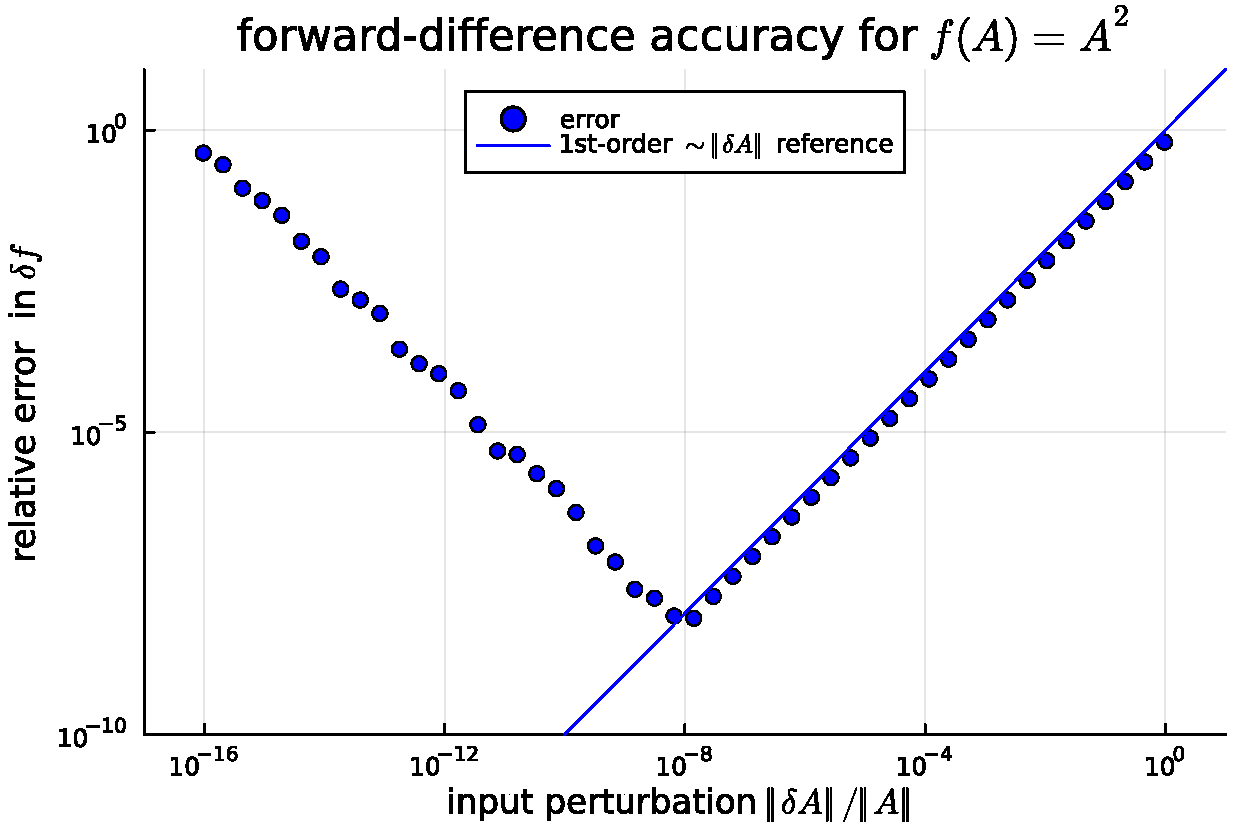
\includegraphics[width=0.8\textwidth]{figures/fig1}
    \caption{Forward-difference accuracy for $f(A) = A^2$, showing the relative error in $\delta f = f(A + \delta A) - f(A)$ versus the  linearization $f'(A) \delta A$, as a function of the magnitude $\Vert \delta A\Vert$.  $A$ is a $4 \times 4$ matrix with unit-variance Gaussian random entries, and $\delta A$ is similarly a unit-variance Gaussian random perturbation scaled by a factor $s$ ranging from $1$ to $10^{-16}$.}
\end{figure}

We notice two main features as we decrease $\delta A$:
\begin{enumerate}
    \item The relative error at first decreases linearly with $\lVert \delta A\rVert$. This is called \textbf{first-order accuracy}. Why?
    \item When $\delta A$ gets too small, the error increases. Why?
\end{enumerate}

\subsection{Order of accuracy}

The \textbf{truncation error} is the inaccuracy arising from the fact that the input perturbation $\delta x$ is not infinitesimal: we are computing a difference, not a derivative.
If the truncation error in the derivative scales proportional $\Vert \delta x \Vert^n$, we call the approximation \textbf{n-th order accurate}.  For forward differences, here, the order is \textbf{n=1}.  Why?

For any $f(x)$ with a nonzero second derivative (think of the Taylor series), we have
\begin{displaymath}
	f(x + \delta x) = f(x) + f'(x) \delta x + (\text{terms proportional to }\Vert \delta x \Vert^2) + \underbrace{o(\Vert \delta x \Vert^2)}_\text{i.e. higher-order terms}
\end{displaymath}
That is, the terms we \textit{dropped} in our forward-difference approximations are proportional to $\Vert \delta x\Vert^2$.  But that means that the \textbf{relative error is linear}:
\begin{align*}
	\text{relative error} &= \frac{\Vert f(x+\delta x) - f(x) - f'(x) \delta x \Vert}{\Vert f'(x) \delta x \Vert} \\
	&= \frac{(\text{terms proportional to }\Vert \delta x \Vert^2) + o(\Vert \delta x \Vert^2)}{\text{proportional to }\Vert \delta x \Vert} = (\text{terms proportional to }\Vert \delta x \Vert) + o(\Vert \delta x \Vert)
\end{align*}
This is \textbf{first-order accuracy}.
Truncation error in a finite-difference approximation is the \textbf{inherent} error in the formula for \textbf{non-infinitesimal} $\delta x$.  Does that mean we should just make $\delta x$ as small as we possibly can?

\subsection{Roundoff error}


The reason why the error \textit{increased} for very small $\delta A$ was due to \textbf{roundoff errors}.  The computer only stores a \textbf{finite number of significant digits} (about 15 decimal digits) for each real number and rounds off the rest on each operation — this is called  \href{https://en.wikipedia.org/wiki/Floating-point_arithmetic}{floating-point arithmetic}. If $\delta x$ is too small, then the difference $f(x+\delta x) - f(x)$ gets rounded off to zero (some or all of the \textit{significant digits cancel}).  This is called  \href{https://en.wikipedia.org/wiki/Catastrophic_cancellation}{catastrophic cancellation}.

Floating-point arithmetic is much like scientific notation ${*}.{*}{*}{*}{*}{*} \times 10^e$: a finite-precision coefficient ${*}.{*}{*}{*}{*}{*}$ scaled by a power of~$10$ (or, on a computer, a power of~$2$). The number of digits in the coefficient (the ``significant digits'') is the ``precision,'' which in the usual 64-bit floating-point arithmetic is charactized by a quantity $\epsilon = 2^{-52} \approx 2.22 \times 10^{-16}$, called the \href{https://en.wikipedia.org/wiki/Machine_epsilon}{machine epsilon}.  When an arbitrary real number $y \in \mathbb{R}$ is rounded to the closest floating-point value $\tilde{y}$, the roundoff error is bounded by $|\tilde{y} - y| \le \epsilon |y|$.  Equivalently, the computer keeps only about 15--16 $\approx -\log_{10} \epsilon$ decimal digits, or really $53 = 1 - \log_2 \epsilon$ \emph{binary} digits, for each number. 

In our finite-difference example, for $\Vert \delta A \Vert / \Vert A \Vert$ of roughly $10^{-8} \approx \sqrt{\epsilon} \lVert A\rVert$ or larger, the approximation for $f'(A)$ is dominated by the truncation error, but if we go smaller than that the relative error starts increasing due to roundoff. Experience has shown that $\Vert \delta x \Vert \approx \sqrt{\epsilon} \Vert x \Vert $ is often a good rule of thumb---about half the significant digits is the most that is reasonably safe to rely on---but the precise crossover point of minimum error depends on the function $f$ and the finite-difference method. But, like all rules of thumb, this may not always be completely reliable.

\subsection{Other finite-difference methods}

There are more sophisticated finite-difference methods, such as Richardson extrapolation, which consider a sequence of progressively smaller $\delta x$ values in order to adaptively determine the best possible estimate for $f'$ (\emph{extrapolating} to $\delta x \to 0$ using progressively higher degree polynomials).   One can also use higher-order difference formulas than the simple forward-difference method here, so that the truncation error decreases faster than than linearly with $\delta x$.  The most famous higher-order formula is the ``centered difference'' $f'(x) \delta x \approx [f(x + \delta x) - f(x - \delta x)]/2$, which has \emph{second}-order accuracy (relative truncation error proportional to $\Vert \delta x\Vert^2$).  

Higher-dimensional inputs  $x$ pose a fundamental computational challenge for finite-difference techniques, because if you want to know what happens for every possible direction $\delta x$ then you need many finite differences: one for each dimension of $\delta x$. For example, suppose $x \in \mathbb{R}^n$ and $f(x) \in \mathbb{R}$, so that you are computing $\nabla f \in \mathbb{R}^n$; if you want to know the whole gradient, you need $n$ \emph{separate} finite differences.
The net result is that finite differences in higher dimensions are expensive, quickly becoming impractical for high-dimensional optimization (e.g. neural networks) where $n$  might be huge.  On the other hand, if you are just using finite differences as a check for bugs in your code, it is usually sufficient to compare $f(x+\delta x) - f(x)$ to $f'(x)[\delta x]$ in a few random directions, i.e.~for a few random small $\delta x$.